\documentclass{article}

\usepackage[utf8]{inputenc}
\usepackage[T1]{fontenc}% optional T1 font encoding
\usepackage[%
    colorlinks=true,
    pdfborder={0 0 0},
    linkcolor=red
]{hyperref}
\usepackage[all]{hypcap}
\usepackage{amsmath}
\interdisplaylinepenalty=2500
\usepackage{graphicx}
\usepackage[cmintegrals]{newtxmath}
\usepackage{cite}
\usepackage{listings}
\usepackage{hyperref}
\usepackage{indentfirst}

\begin{document}

\title{MC 613 - Diagrama de Blocos}
\author{Luiz Eduardo T. C. Cartolano(RA 183012)
        e Yago de Lima Barbosa(RA 188727) }
\date{Maio 2018}

\maketitle

\section{Introdução}
O jogo da velha se popularizou na Inglaterra do século XIX \cite{ref:velha-hist}, sendo jogado, especialmente, por mulheres de idade mais avançada. Contudo, dizem que as origens do jogo são mais antigas, escavações realizadas no templo de Kurna, no Egito, encontraram referências a ele que datavam do século 14 antes de Cristo. Mas outros achados arqueológicos comprovam que o jogo da velha e muitos outros passatempos similares foram desenvolvidos independentemente nas mais diferentes regiões do planeta: ele também era jogado na China antiga, na América pré-colombiana e no Império Romano, entre outros.

Grande parte da popularidade do jogo se dá pela facilidade que ele apresenta, o conjunto de regras\cite{ref:velha-regras} que o rege é extremamente simples. Basicamente, os jogadores jogam alternadamente, o objectivo é conseguir três círculos ou três xis em linha, quer horizontal, vertical ou diagonal.

\section{Descrição do projeto}
Na implementação do projeto, seguiremos o seguinte esquema: o jogador utiliza o mouse para marcar sua opção no monitor. O jogo deve permitir escolher qual jogador começa e jogar contra outro ser humano em turnos ou contra uma IA, que obrigatoriamente deve ganhar sempre que possível (o jogo da velha é determinístico). Ao terminar o jogo, mostramos no monitor quem foi o vencedor (ou o empate caso não tenha um) e forneceremos a opção de se iniciar um novo jogo.


\section{Diagrama de Blocos}
O diagrama de blocos para o projeto do Jogo da velha que será implementado pode ser visto na Figura \ref{fig:diagrama}, ele foi criado usando uma ferramenta para desenhos de diagramas do Google e pode ser acessado clicando \href{https://drive.google.com/file/d/1U_X492n2xRLVOVa0kffrWD5SYa2kWRCx/view?usp=sharing}{aqui}. Nele as setas representam dados e os conectores sinais de controles. Uma descrição mais detalhada de cada um dos blocos é dada a seguir.
    \subsection{Bloco Mouse}
        \begin{itemize}
            \item \textbf{Entradas:} Dados recebidos na entrada PS2 da placa(de I/O).
            \item \textbf{Saída:} Posição atual do mouse(para Monitor), dados iniciais da partida(para MJ) e jogada do turno(para MJ).
            \item \textbf{Função:} Gerenciar as ações a serem tomadas pelo clique do mouse, além de coletar e processar os dados do mouse.
        \end{itemize}

    \subsection{Bloco Monitor}
        \begin{itemize}
            \item \textbf{Entradas:} Posição do mouse(de Mouse) e situação atual do jogo(de MJ).
            \item \textbf{Saída:} Imagem atualizada do jogo(pintura dos pixels) para a porta VGA da placa(I/O).
            \item \textbf{Função:} Manter a tela do jogo atualizada no monitor VGA.
        \end{itemize}

    \subsection{BlocoMJ - Memória do Jogo}
        \begin{itemize}
            \item \textbf{Entradas:} Dados iniciais do jogo(de Mouse) e as jogadas(de Mouse e IA).
            \item \textbf{Saída:} Situação do \emph{grid} e dados inicias do jogo (para IA, Monitor e Mouse).
            \item \textbf{Função:} Armazenar os dados e situação do jogo(fase do jogo, preenchimento do \emph{grid} e dados iniciais do jogo).
        \end{itemize}

    \subsection{Bloco IA - Inteligência Artificial}
        \begin{itemize}
            \item \textbf{Entradas:} Situação do grid do jogo(de MJ).
            \item \textbf{Saída:} Melhor jogada para a situação atual do jogo(para MJ).
            \item \textbf{Função:} Verificar a melhor jogada possível, de forma a ganhar sempre que puder.
Entrada: Situação do grid do jogo(de MJ).
        \end{itemize}

    \subsection{Bloco UC - Unidade de Controle}
        \begin{itemize}
            \item \textbf{Função:} Controlar o fluxo de dados do projeto: permitir que a memória(MJ) seja lida ou gravada, acionar a atualização da tela(Monitor), acionar a jogada da IA .
        \end{itemize}

\begin{figure}[h!]
    \centering
    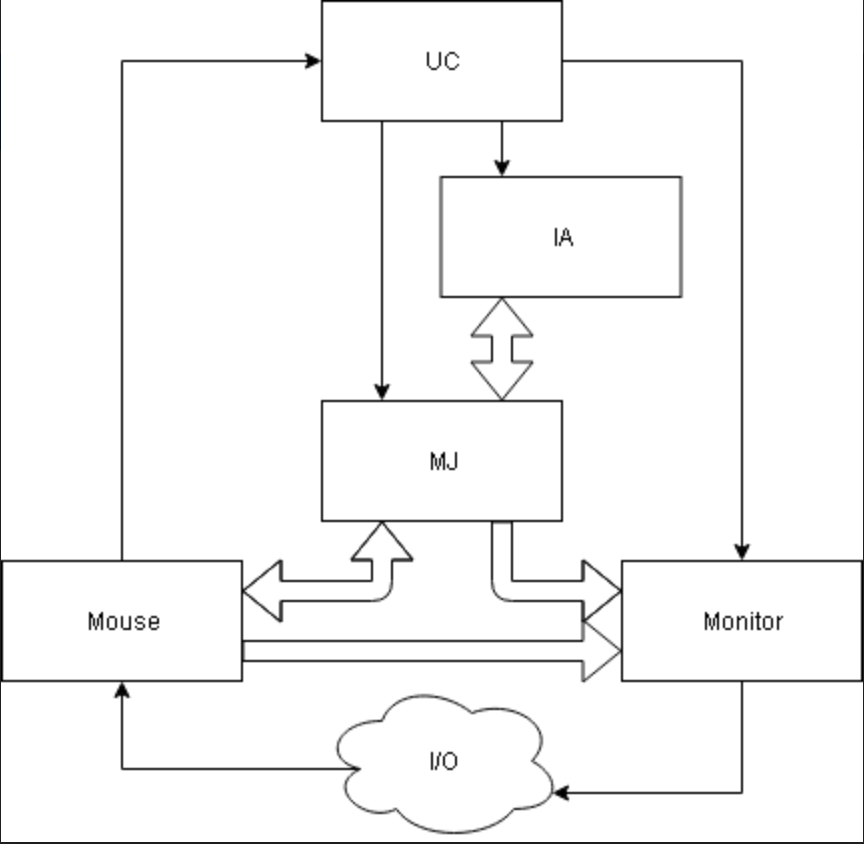
\includegraphics[scale=0.7]{diagrama.png}
    \caption{\label{fig:diagrama}Diagrama de blocos para o projeto de Jogo da Velha da disciplina de MC613.}
\end{figure}


\nocite{*}
\bibliographystyle{plain}
\bibliography{references}

\end{document}
